Se realizó un programa que calcula el área y perímetro de dos figuras geométricas: el trapecio y triángulo. Para ello se reciben datos del usuario mediante la herramienta \emph{Textbox} y se muestran los resultados mediante la herramienta \emph{Label}.

\textbf{Trapecio:} para calcular el área se utilizó la fórmula del área del trapecio. Para el perímetro se calculó la longitud del lado diagonal mediante el teorema de pitágoras y se sumó con los otros 2 lados y la base.

\textbf{Área del trapecio:}

\begin{equation*}
  Área = \frac{Altura 1 + Altura 2}{2} * Base
\end{equation*}

\textbf{Perímetro del trapecio:}

\begin{equation*}
  Perímetro = Lado1 + Lado2 + Base + Lado3
\end{equation*}

\textbf{Triángulo:} para calcular el área se emplea la fórmula de área del triángulo. Para el perímetro se suman los dos lados y la base.

\textbf{Área del triángulo:}

\begin{equation*}
  Área = \frac{Base * Altura}{2}
\end{equation*}

\textbf{Perímetro del triángulo:}

\begin{equation*}
  Perímetro = Lado1 + Lado2 + Base
\end{equation*}

\textbf{Código del programa:}

código

\textbf{Captura de ejecución:}

\begin{figure}[H]
  \centering
  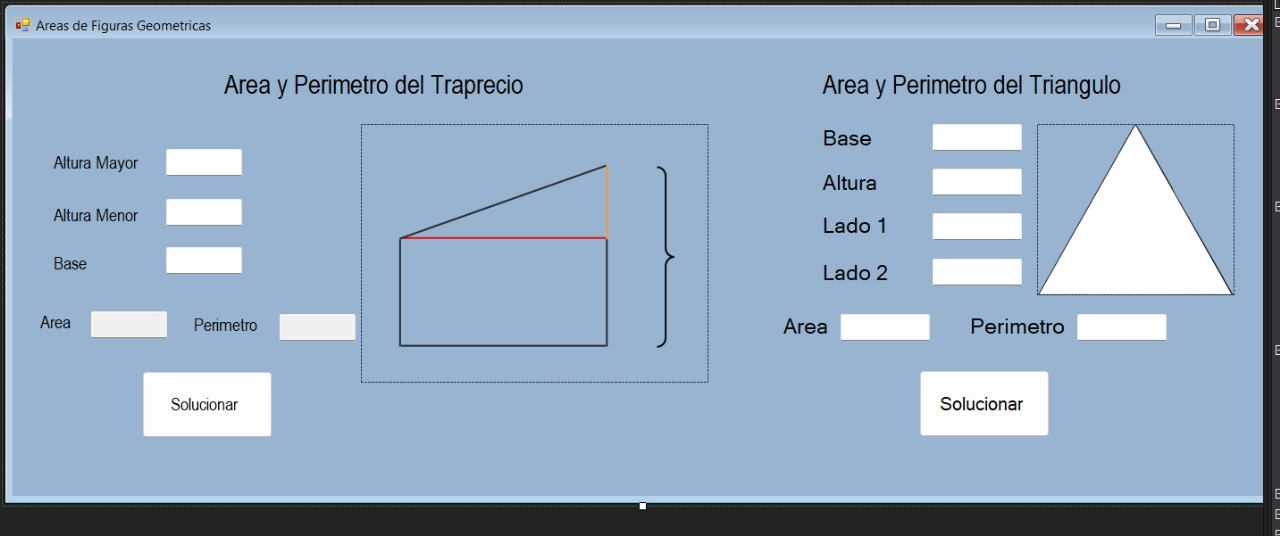
\includegraphics[scale = 0.5]{Imagenes/interfaz_grafica.jpeg}
  \caption{Interfaz Gráfica}{Fuente: Propia}
\end{figure}